\chapter{Código ColorADD} \label{coloradd}


\begin{figure}[ht]
\begin{minipage}[b]{0.45\linewidth}
\centering

\includegraphics[width=\textwidth]{coloradd}
    \caption{Código ColorADD}
    \label{fig:coloradd}
\end{minipage}
\hspace{0.5cm}
\begin{minipage}[b]{0.45\linewidth}
\centering
    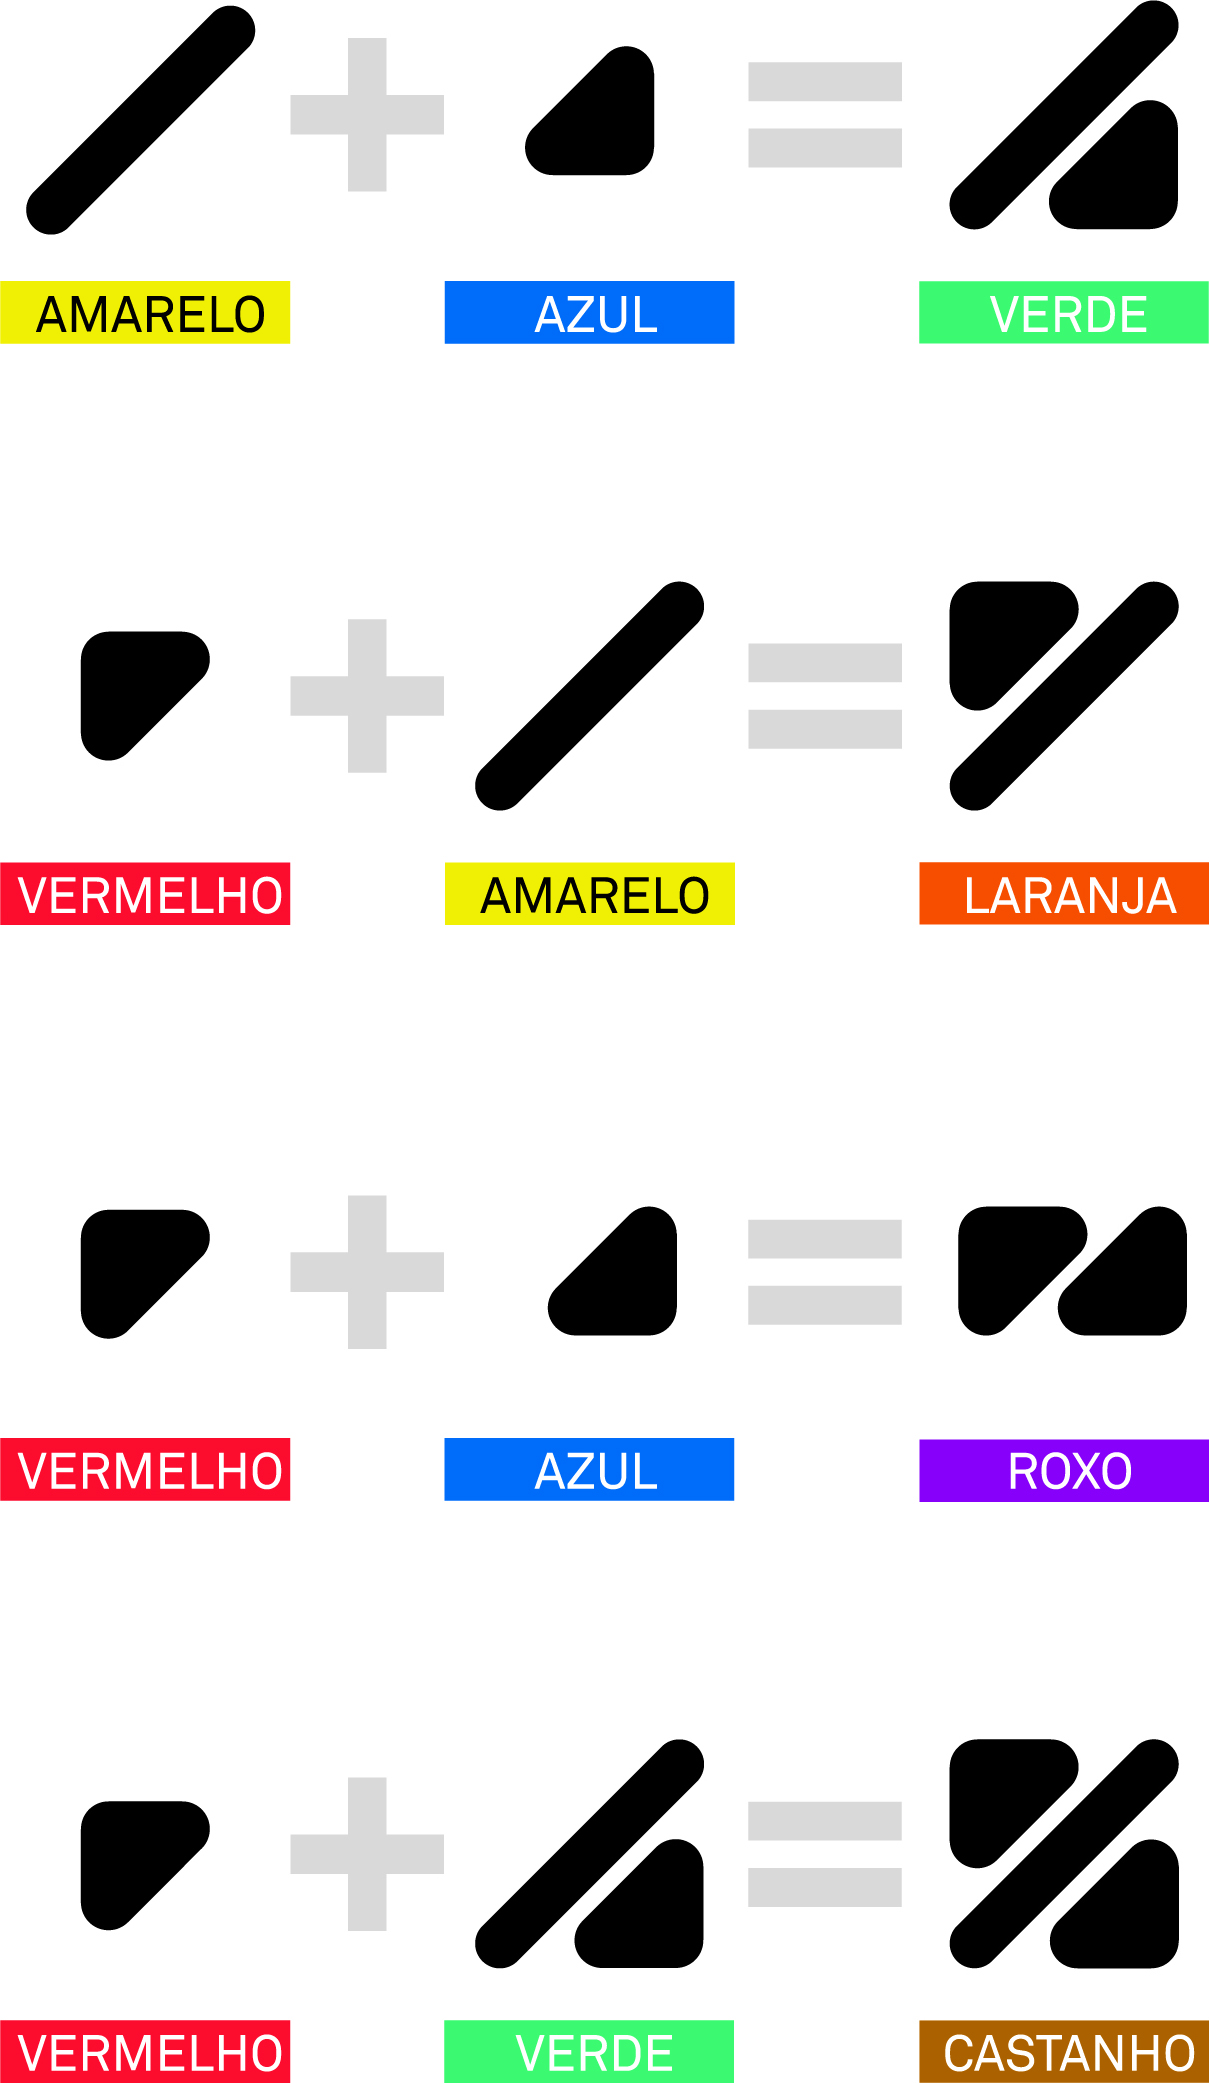
\includegraphics[width=\textwidth]{coloradd_como}
    \caption{Adição de cores ColorADD}
    \label{fig:coloradd_como}
\end{minipage}
\end{figure}

\begin{figure}[t]
  \begin{center}
    \leavevmode
    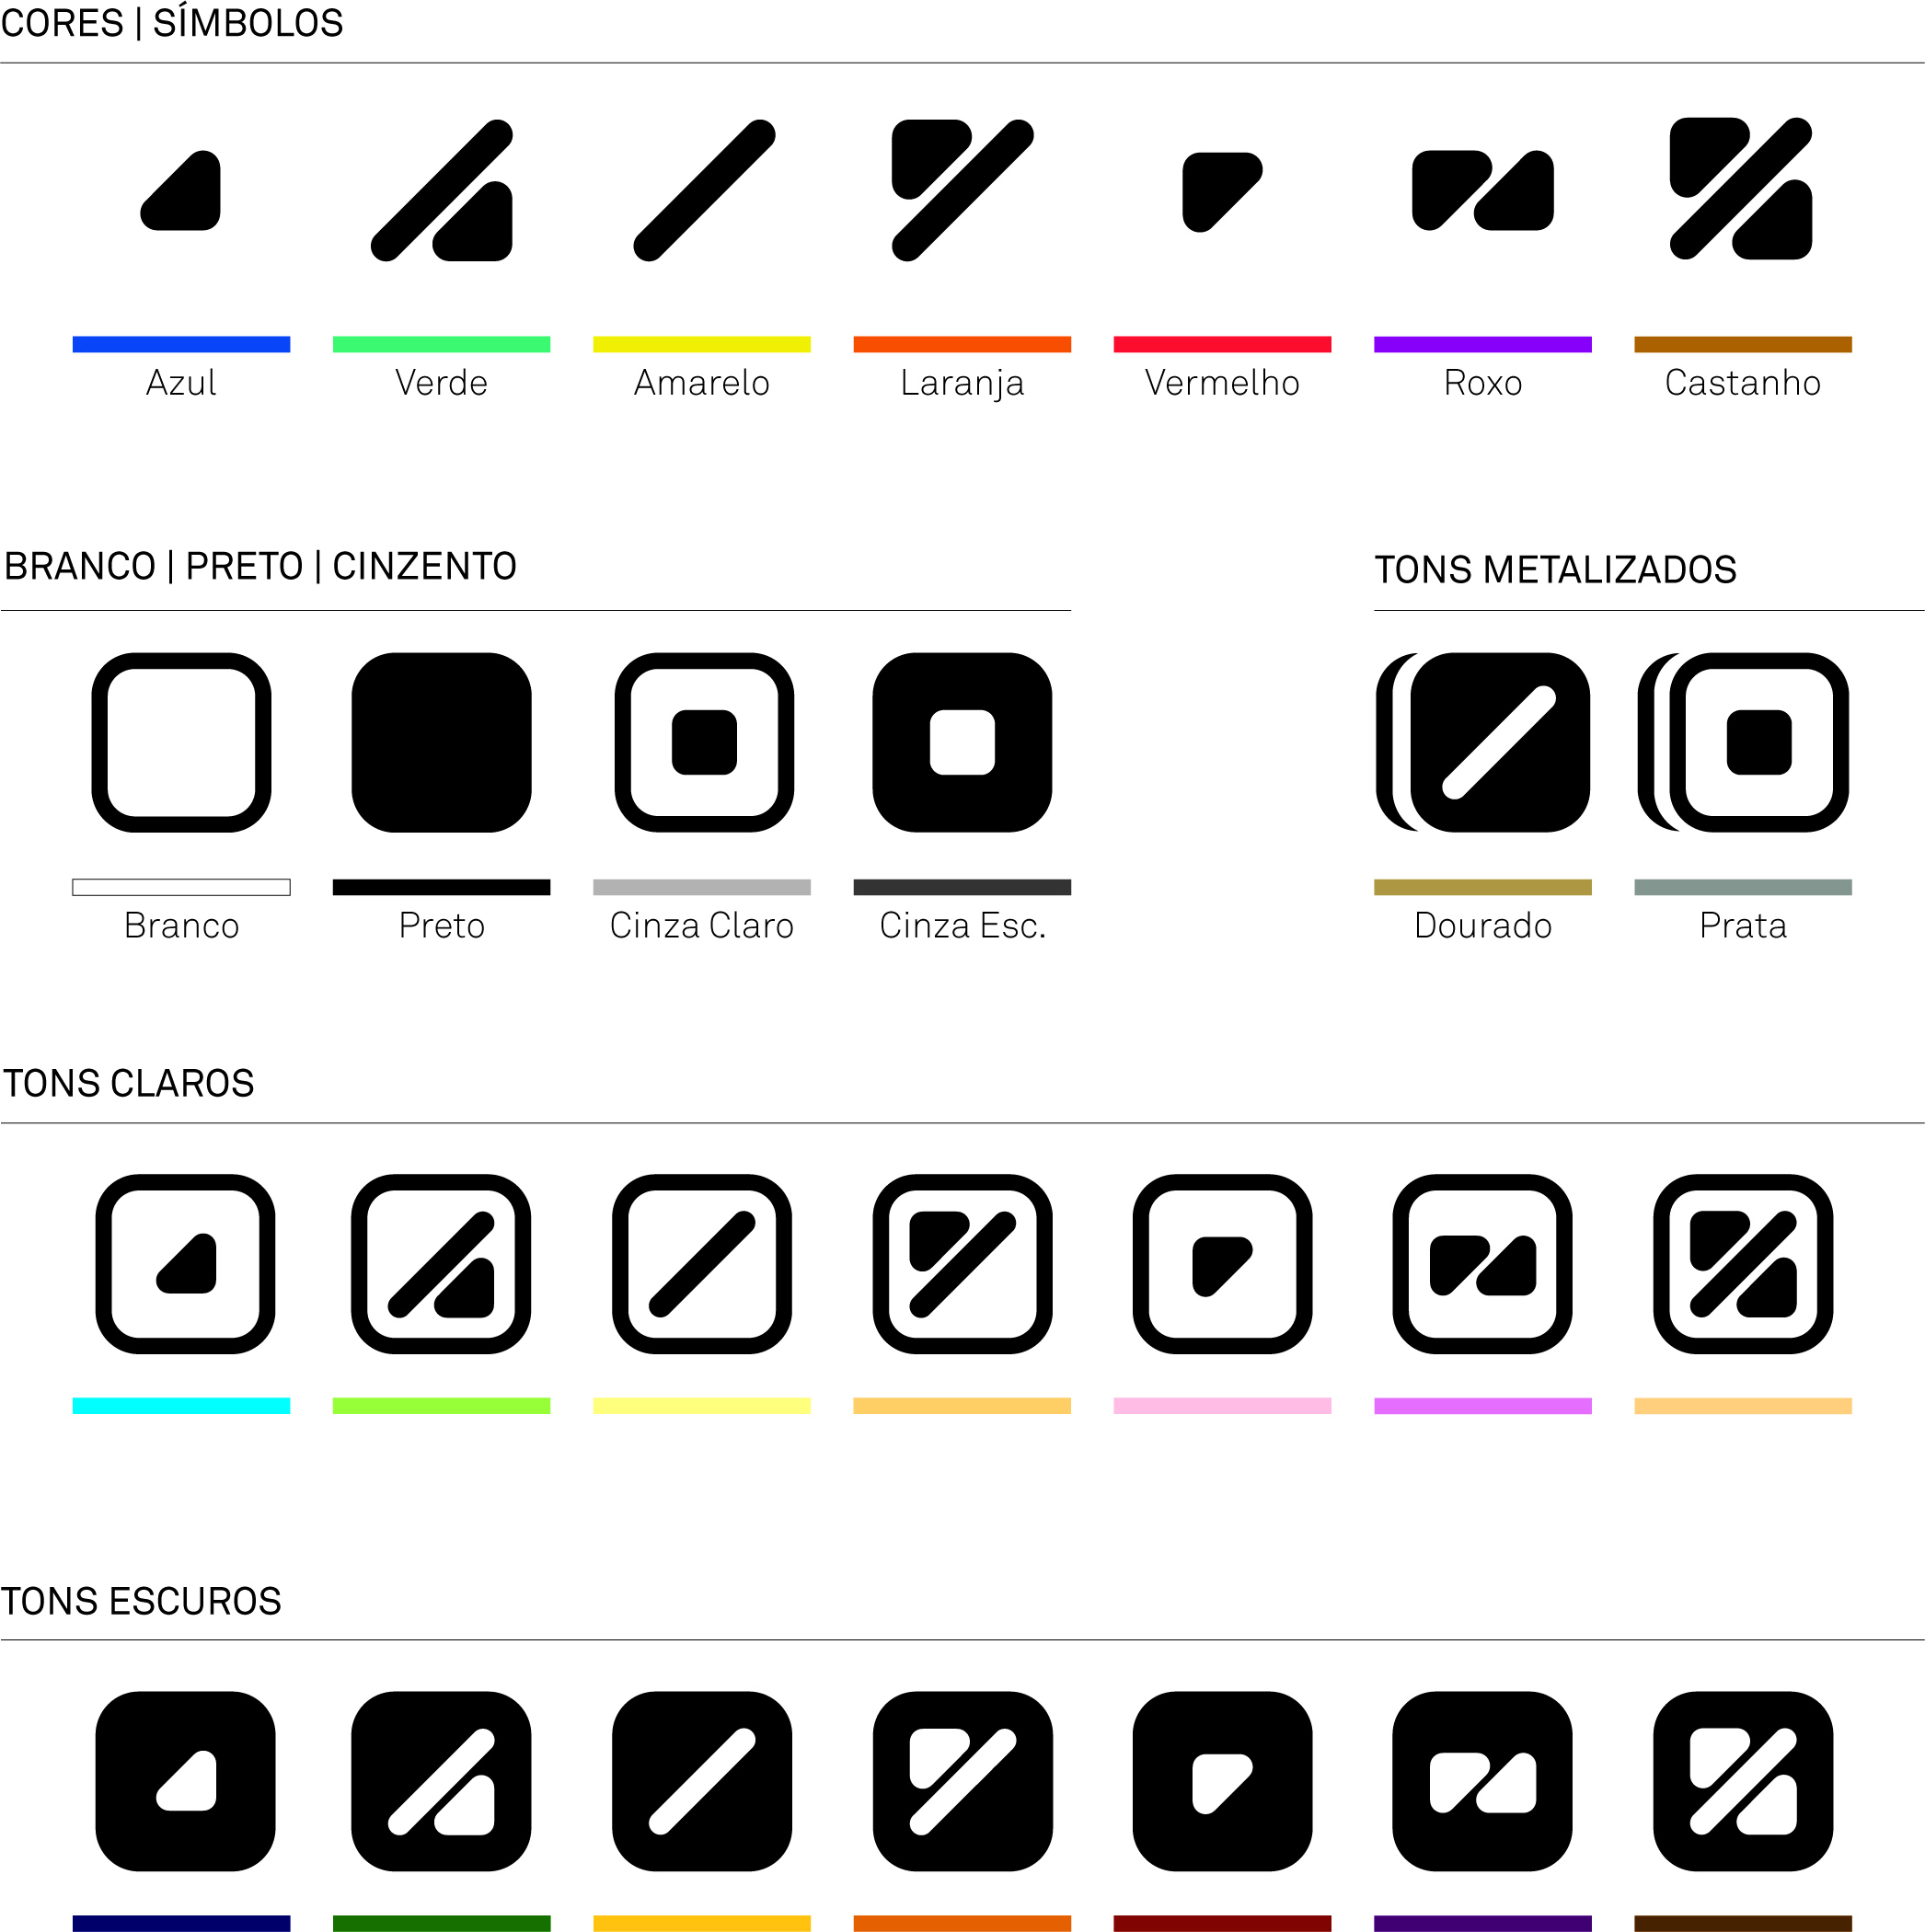
\includegraphics[width=\textwidth]{coloradd_tabela}
    \caption{Tabela de cores ColorADD}
    \label{fig:coloradd_tabela}
  \end{center}
\end{figure}
